\providecommand{\relativeRoot}{../..}
\documentclass[\relativeRoot/main.tex]{subfiles}
\graphicspath{
    {\subfix{./figures/}}
}

\begin{document}

\section{The Lymphatic System}
\label{sec:intro:lymph_system}

\begin{figure}
    \centering
    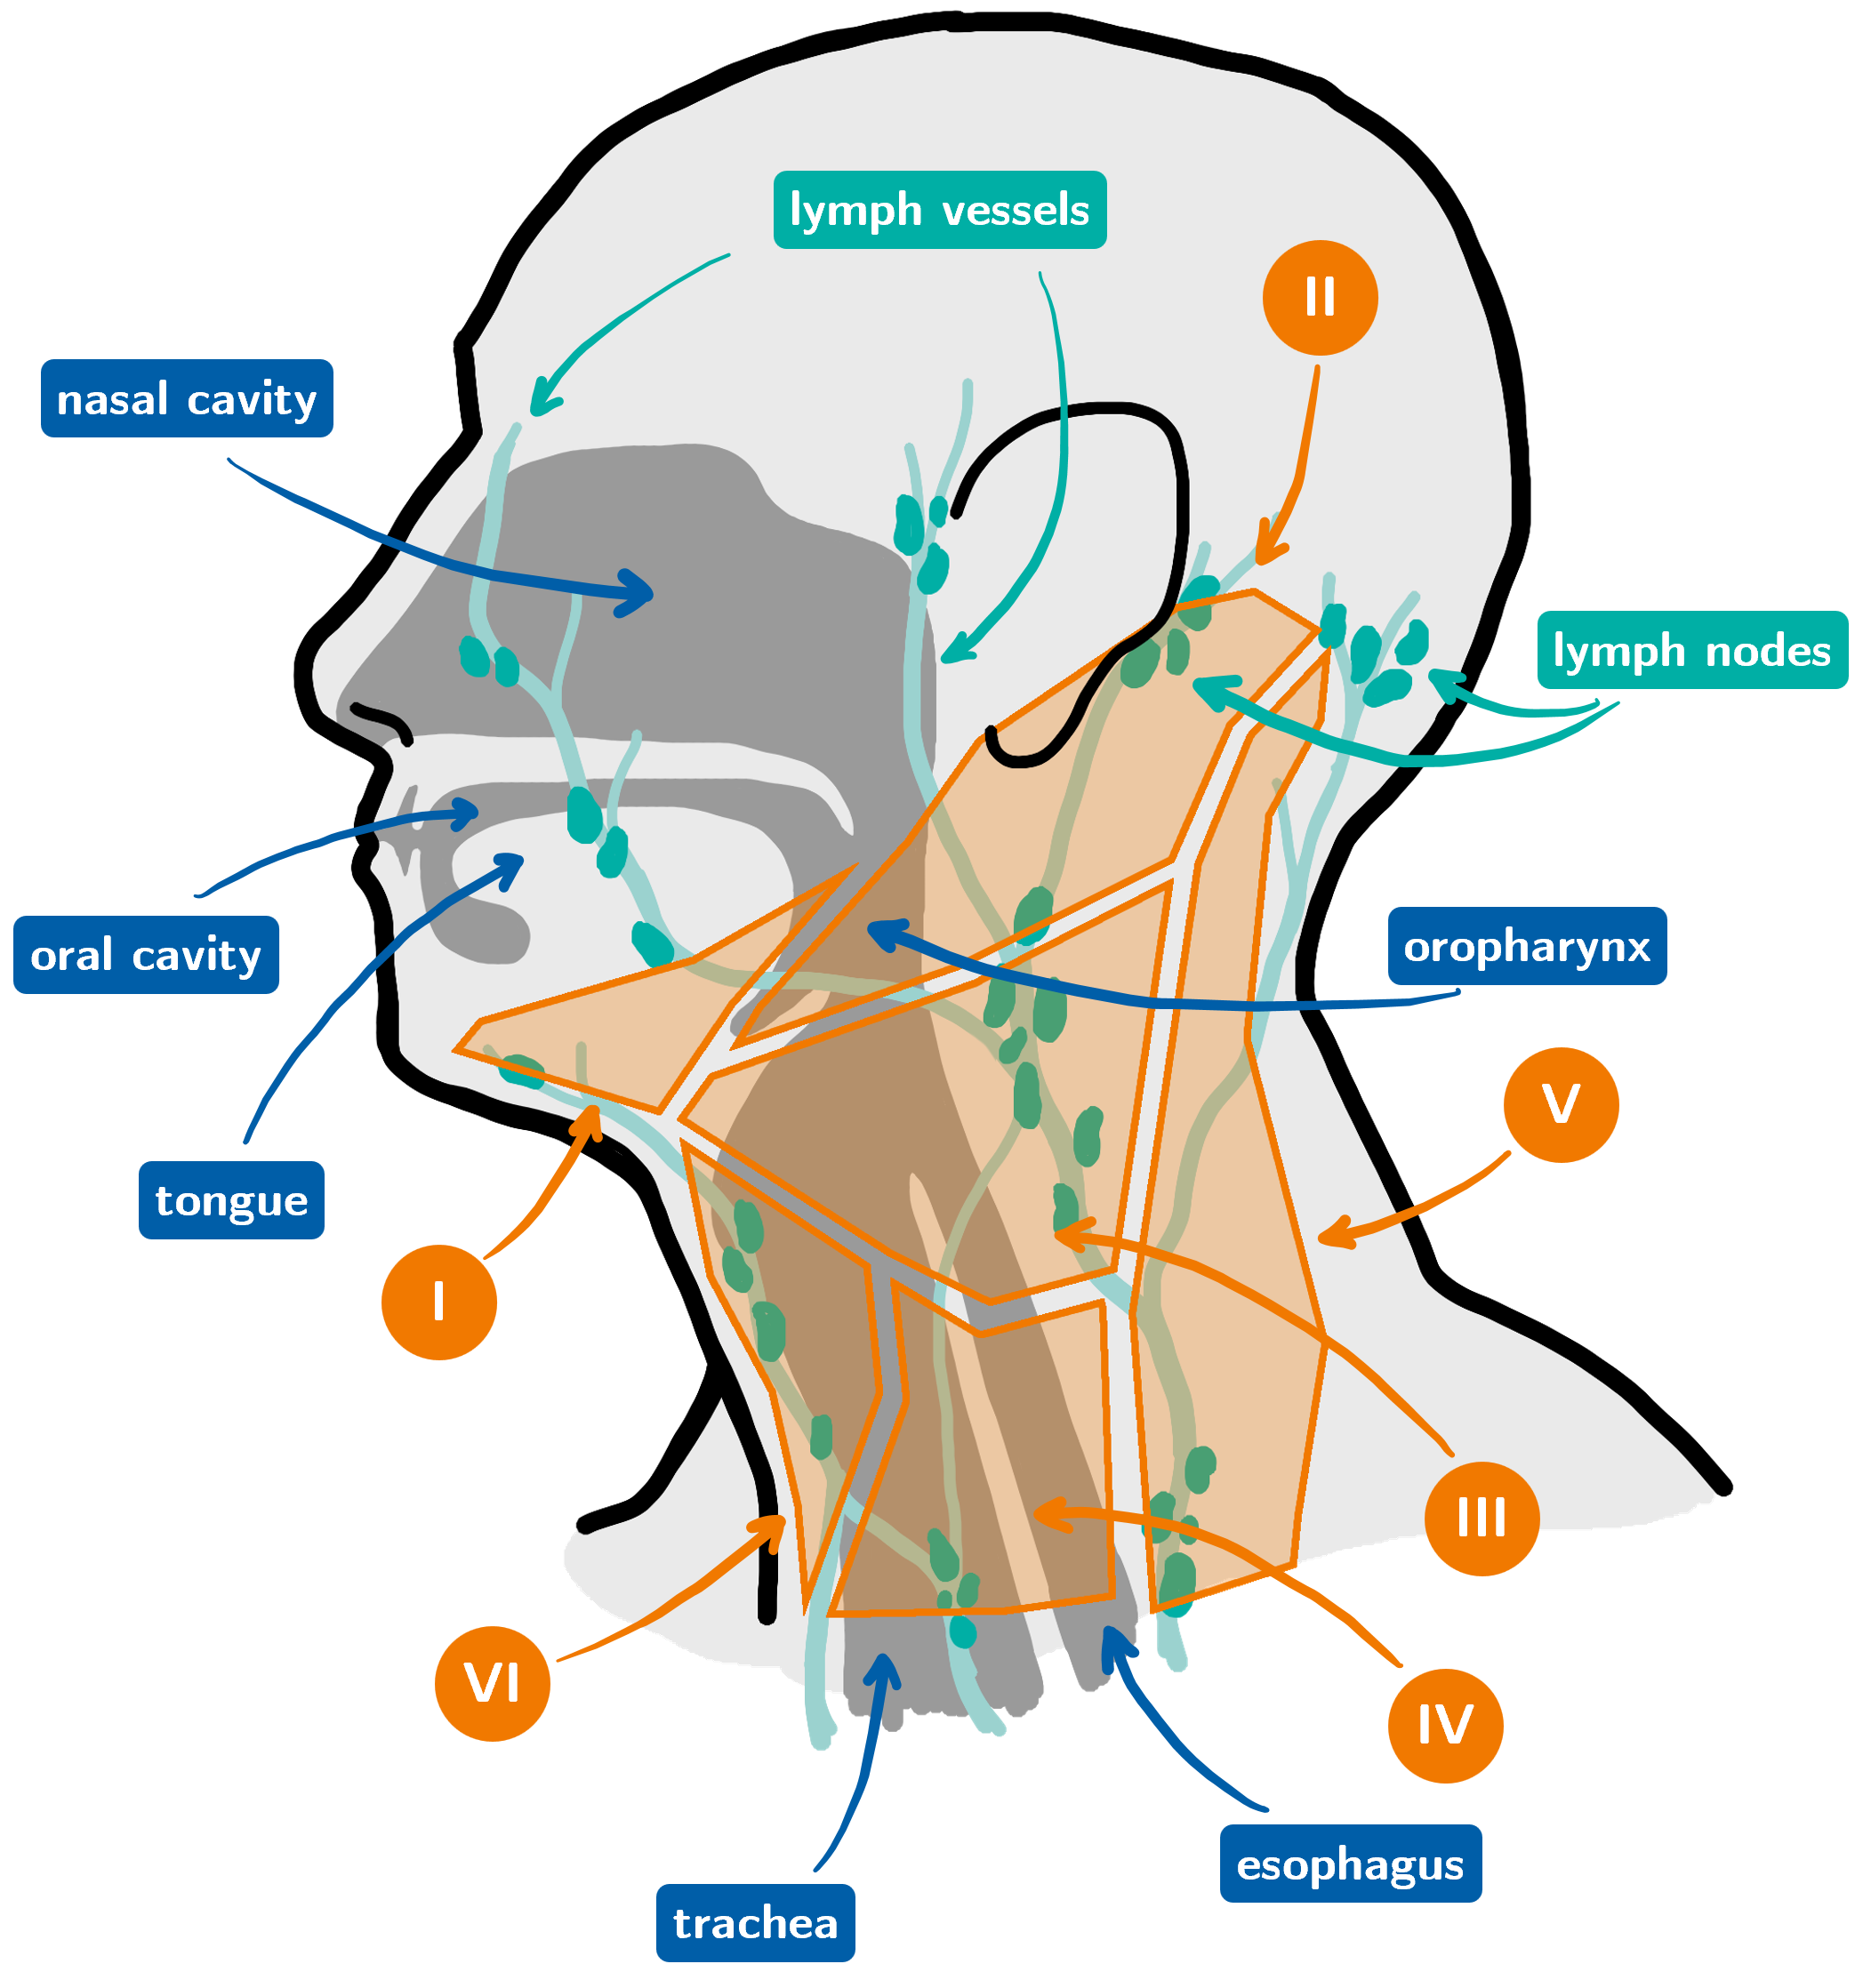
\includegraphics[width=\textwidth]{figures/head_and_neck_labelled.png}
    \caption[
        Schematic drawing of the head and neck region.
    ]{
        Schematic drawing of the lymphatic network in the head and neck region. The shaded area in dark gray depicts a sagittal cross-section of the upper respiratory track and is labelled with blue arrows and tags. Lymphatic vessels are drawn in light green with dark green lymph nodes attached to them. On top, using a transparent shade of orange and orange outlines, we have roughly indicated the location of the \glspl{lnl}. They group the lymph nodes in the head and neck region into regions that are separated by anatomical features not shown in this schematic. E.g., the inferior border of the hyoid bone separates \gls{lnl} II and III axially. The diagram has been roughly traced from the anatomical illustrations in \citeauthorandlink{lengele_anatomical_2007}.
    }
    \label{fig:intro:schematics_head}
\end{figure}



\end{document}